\section{Experiments and Results}

 \frame{\sectionpage}

 \begin{frame}{An Overview}
    \begin{table}[h!]
        %\small
        \begin{center}
            \begin{tabular}{lccc}
            
            & \multicolumn{2}{c}{{\textbf{report}}} & \multirow{2}{*}{{\textbf{no report}}} \\
            & {\textit{ \textcolor{fuzzywuzzy!65!white}{shareable}}} & {\textit{non-shareable}} & \\
            \hline
            \multirow{2}{*}{{\color{fuzzywuzzy!65!white} \underline{No. certified applicants}}} & \multicolumn{2}{c}{{seeker $\textcolor{fuzzywuzzy!65!white}{+}$ / eqbm $\textcolor{fuzzywuzzy!65!white}{+}$}} & {0} \\
             & {seeker $\textcolor{fuzzywuzzy!65!white}{+}$ {$\textcolor{fuzzywuzzy!65!white}{\boxed{\searrow}}$} / eqbm $\textcolor{fuzzywuzzy!65!white}{+}$} & {seeker $\textcolor{fuzzywuzzy!65!white}{+}$ / eqbm $\textcolor{fuzzywuzzy!65!white}{\sim 0}$} & 
            \end{tabular}
        \end{center}
    \end{table}
 \end{frame}

\subsection*{Experiment I}
\begin{frame}{Intervention 1: Shareable Credible Assessments}
    \begin{table}[h!]
        \scriptsize
        \begin{center}
            \begin{tabular}{lccc}
            
            & \multicolumn{2}{c}{{\textbf{report}}} & \multirow{2}{*}{{\textbf{no report}}} \\ %\color{gray!80!black}
            & {{\textbf{shareable}}} & {\transparent{0.2}\textit{non-shareable}} & \\
            \hline
            \multirow{2}{*}{\transparent{0.2}{\color{fuzzywuzzy!65!white} \underline{No. certified applicants}}} & \multicolumn{2}{c}{?} & {0} \\
             & {\transparent{0.2}{?}} & {\transparent{0.2}?} & 
            \end{tabular}
        \end{center}
    \end{table}
    \vspace*{-5pt}
    \begin{itemize}
        \small
        \item[\texthlit{T1}] email version, and 20+ colorered high-quality paper copies\uncover<2->{ \texthlbf{with credibility}} 
    \end{itemize}

    \vspace*{-18pt}
    \begin{columns}[T]
        \begin{column}{0.4\textwidth}
            \begin{figure}
                \centering
                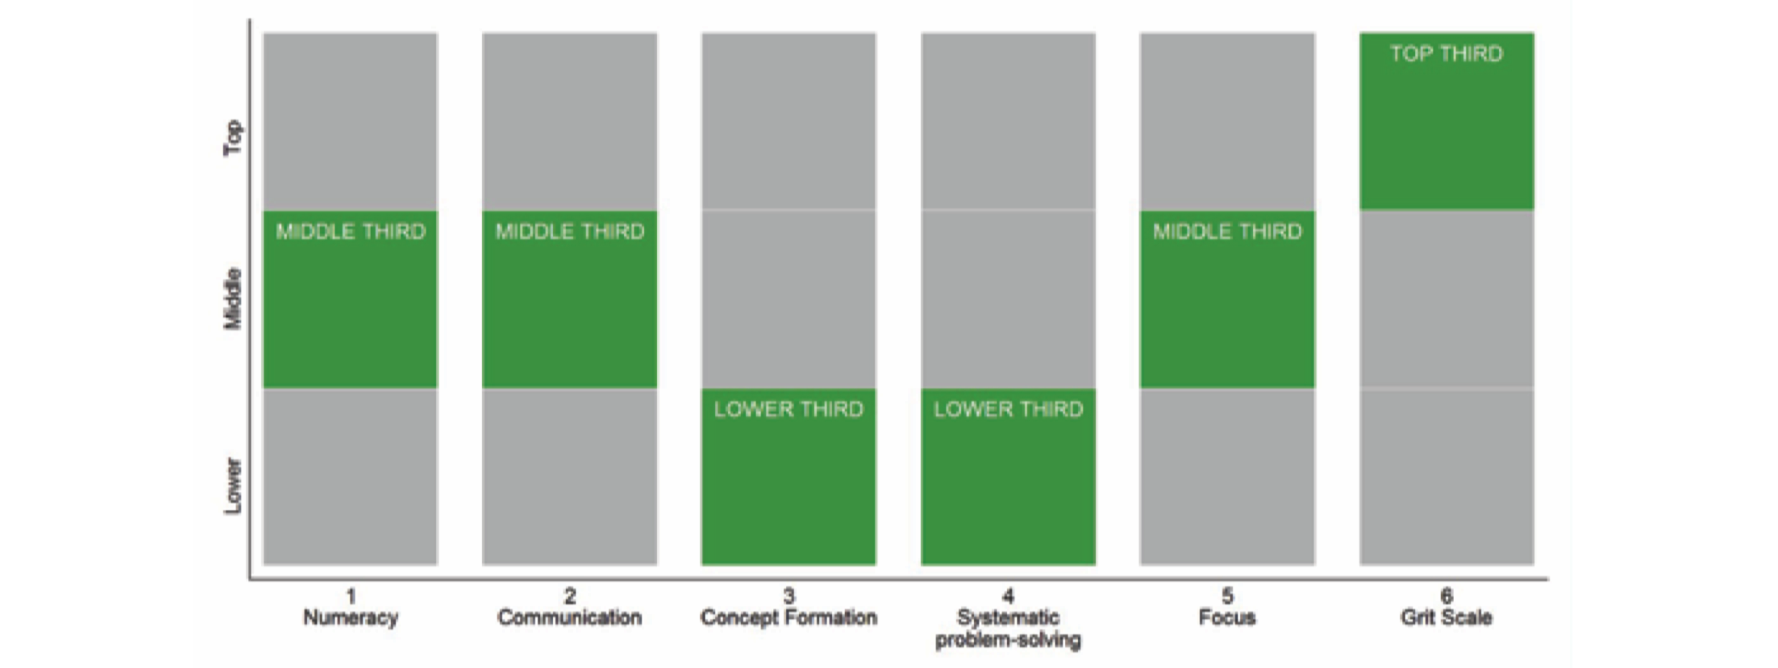
\includegraphics[width = 0.95 \textwidth]{images/T1_assess.png}
            \end{figure}
        \end{column}

        \begin{column}{0.55\textwidth}
            \uncover<2->{\begin{figure}
                \centering
                
\includegraphics[width = 0.95 \textwidth]{images/T1_cert.png}
            \end{figure}}

            \uncover<3>{
            \vspace*{-15pt}
            \begin{itemize}
                \footnotesize
                \item[-] assessments are carefully explained
                \item[-] encouraged to be used for job application
            \end{itemize}
            }
        \end{column}
    \end{columns}

\end{frame}

\begin{frame}{Intervention 1: Shareable Credible Assessments}
    \vspace*{-5pt}
    \begin{itemize}
        \small
        \item[\texthlit{T1}] email version, and 20+ colorered high-quality paper copies\uncover<2->{ \texthlbf{with credibility}} 
    \end{itemize}
    \begin{table}[h!]
        \small
        \begin{center}
            \begin{tabular}{lccc}
            
            & \multicolumn{2}{c}{{\textbf{report}}} & \multirow{2}{*}{{\textbf{no report}}} \\
            & {{\textbf{shareable}}} & {\transparent{0.2}\textit{non-shareable}} & \\
            \hline
            \multirow{2}{*}{\transparent{0.2}{\color{fuzzywuzzy!65!white} \underline{No. certified applicants}}} & \multicolumn{2}{c}{?} & {0} \\
             & {\transparent{0.2}{?}} & {\transparent{0.2}?} & \\ \hline \hline
            N & \multicolumn{2}{c}{\textbf{2247}} & \textbf{2274}
            \end{tabular}
        \end{center}
    \end{table}
    {\small Both T and C groups received job searching counseling and tips, a CV template, interview tips}
    
\end{frame}

\begin{frame}{Intervention 1: Estimation}
    $$
    Y_{id} = \mathbf{T}_d\cdot\Delta +\mathbf{X}_{id}\cdot\Gamma + S_d+\epsilon_{id}
    $$
    where
    \begin{itemize}
        \small
        \item[$\textcolor{fuzzywuzzy!65!white}{Y_{id}}$]: outcome for workseeker $i$ assessed on date $d$
        \item[$\textcolor{fuzzywuzzy!65!white}{\mathbf{T}_{d}}$]: treatment assignments
        \item[$\textcolor{fuzzywuzzy!65!white}{\mathbf{X}_{id}}$]: prespecified baseline covariates {\footnotesize(some unbalanced variables don't affect results)}
        \item[$\textcolor{fuzzywuzzy!65!white}{S_{d}}$]: block fixed effects {\footnotesize(days of treatment randomly assigned within blocks)} 
        \item[$\textcolor{fuzzywuzzy!65!white}{\epsilon_{id}}$]: robust standard errors clustered at assessment date level
    \end{itemize}
\end{frame}

\begin{frame}{Intervention 1: Treatment Effects}
    \begin{table}[h!]
        \footnotesize
        \begin{center}
            \begin{tabular}{lccccc}
            & Employed & Hours & Earnings & Hourly wage & Written contract \\
            \hline
            treatment & $0.052^{***}$ & \textcolor<2->{fuzzywuzzy!65!white}{$0.201^{***}$} & \textcolor<2->{fuzzywuzzy!65!white}{$0.337^{***}$} & \textcolor<2->{fuzzywuzzy!65!white}{$0.197^{***}$} & \textcolor<2->{fuzzywuzzy!65!white}{$0.020^{**}$}\\
             &\\
             mean outcome & 0.309 & 8.848 & 159.291 & 9.840 & 0.120 \\
             mean outcome $\vert$ employed & & 28.847 & 518.291 & 32.283 & 0.392
            \end{tabular}
        \end{center}
    \end{table}
    
    \uncover<2->{
        A decomposition:
        \footnotesize
        \begin{align*}
        &\mathbb{E}\left[ \text{Earn}\mid \text{Treat}=1\right]- \mathbb{E}\left[ \text{Earn}\mid \text{Treat}=0\right] & \text{ATE} \\
        =& \underbrace{\left( \mathbb{E}\left[ \text{Earn}\mid \text{Treat}=1,\text{Work}=1\right] - \mathbb{E}\left[ \text{Earn}\mid \text{Treat}=0,\text{Work}=1\right] \right)}_{ \uncover<3->{\textcolor<3>{fuzzywuzzy!65!white}{\text{ATE for earnings }\mid\text{ employed}}} } \cdot \underbrace{\Pr \left[ \text{Work}=1\mid \text{Treat}=1\right]}_{ \uncover<3->{\textcolor<3>{fuzzywuzzy!65!white}{\text{Treated employment rate}}} } & \uncover<3->{\text{IM}} \\
        &+ \underbrace{\mathbb{E}\left[ \text{Earn}\mid \text{Treat}=0,\text{Work}=1\right]}_{\uncover<4->{\textcolor<4>{fuzzywuzzy!65!white}{\text{Control earnings }\mid\text{ employed}}}} \cdot \underbrace{\left( \Pr \left[ \text{Work}=1\mid \text{Treat}=1\right]-\Pr \left[ \text{Work}=1\mid \text{Treat}=0\right] \right)}_{\uncover<4->{\textcolor<4>{fuzzywuzzy!65!white}{\text{ATE for employment}}}} & \uncover<4>{\text{EM}}
    \end{align*}}
\end{frame}

\begin{frame}{Intervention 1: Treatment Effect Decomposition}
    \vspace*{-10pt}
    {\footnotesize 
    \begin{align*}
        \text{ATE} = &\left(\textcolor<6>{fuzzywuzzy!65!white}{\text{ATE for earnings} \mid \text{employed}}\right)\cdot \left(\text{Treated employment rate}\right) & \textcolor<3>{fuzzywuzzy!65!white}{\text{IM}}\\
        & \left( \text{Control earnings} \mid \text{employed} \right) \cdot \left( \text{ATE for employment} \right) & \textcolor<2>{fuzzywuzzy!65!white}{\text{EM}}
    \end{align*}
    }
    \vspace*{-20pt}
    \begin{table}[h!]
        \footnotesize
        \begin{center}
            \begin{tabular}{lccccc}
            & Employed & Hours & Earnings & Hourly wage & Written contract \\
            \hline
            total effect & $\textcolor<6>{fuzzywuzzy!65!white}{0.052^{***}}$ & {$0.201^{***}$} & {$0.337^{***}$} & {$0.197^{***}$} & {$0.020^{**}$}\\
            mean outcome & \textcolor<6>{fuzzywuzzy!65!white}{$0.309$}  \\
            \uncover<2->{extensive margin & & $0.188^{***}$ & $0.269^{***}$ & $0.141^{***}$ & $0.020^{***}$ }\\
            \uncover<5->{intensive margin & & $0.013$ & $0.069^*$ & $0.056^{**}$ & $-0.000$}\\
            \uncover<6->{treatment effect $\mid$ employed &  & $0.037$ & $0.194^{*}$ & $0.158^{**}$ & $-0.001$ }
            \end{tabular}
        \end{center}
    \end{table}
    \vspace*{-5pt}
    \begin{itemize}
        \footnotesize 
        \item<2->[\texthlit{EM}]: ATE on \textbf{\color{fuzzywuzzy!65!white} employment}, priced at the mean earnings in the \textbf{\color{fuzzywuzzy!65!white} control group}
        \item<3->[\texthlit{IM}]: ATE on \textbf{\color{fuzzywuzzy!65!white} wage} conditional on employment {$$\mathbb{E}\left[ \text{Earn}\mid \text{Treat}=1,\text{Work}=1\right] - \mathbb{E}\left[ \text{Earn}\mid \text{Treat}=0,\text{Work}=1\right]$$} \textbf{\color{fuzzywuzzy!65!white} not identified}. \uncover<4->{But \textbf{\color{fuzzywuzzy!65!white}IM=ATE-EM} $\rightarrow$ Delta method}
    \end{itemize}
    \vspace*{10pt}
\end{frame}

\begin{frame}{Intervention 1: Treatment Effect Decomposition}
    \vspace*{-10pt}
    \begin{columns}[T]
        \begin{column}{0.55\textwidth}
            \begin{table}[h!]
                \scriptsize
                \begin{center}
                    \begin{tabular}{lccc}
                    
                    & &\multicolumn{2}{c}{workseekers} \\
                   & & $W_1$ & $W_2$ \\
                    \hline
                    \multirow{2}{*}{jobs} & $J_1$ & $\textcolor{fuzzywuzzy!65!white}{\boxed{P_{1,1}\cdot U(\underbrace{W_{1,1}}_{\leq V_{1,1}})-C}}$ & $P_{2,1}\cdot U(\underbrace{W_{2,1}}_{\leq V_{2,1}})-C$ \\
                    & $J_2$ & $P_{1,2}\cdot U(\underbrace{W_{1,2}}_{\leq V_{1,2}})-C$ & $\textcolor{fuzzywuzzy!65!white}{\boxed{P_{2,2}\cdot U(\underbrace{W_{2,2}}_{\leq V_{2,2}})-C}}$
                    \end{tabular}
                \end{center}
            \end{table}
            When we observe higher wages:
            \begin{itemize}
                \footnotesize
                \item<2-> optimal matching is easier: $P_{i,i}\uparrow$
                \item<3-> \texthlit{latent} output of optimal matches is higher: $V_{i,i}\uparrow$
            \end{itemize}
            \uncover<4->{does $V_{i,i}$ really increase?}
        \end{column}

        \begin{column}{0.4\textwidth}
            \uncover<5->{\begin{table}[h!]
                \scriptsize
                \begin{center}
                    \begin{tabular}{lc}
                    & Employed \\
                    \hline
                    treatment effect & $0.052 \pm 0.024$ \\
                     control & $0.309$ \\
                     \only<6>{\color{fuzzywuzzy!65!white} marginally employed & {\color{fuzzywuzzy!65!white} $0.361 \pm 0.024$}}\only<7->{\color{fuzzywuzzy!65!white} treated outcome & {\color{fuzzywuzzy!65!white} $\left[0.337, 0.385\right]$}}
                    \end{tabular}
                \end{center}
            \end{table}}
            \vspace*{-20pt}
            \only<7>{
                \begin{center}
                    \begin{tikzpicture}[scale=1]
                        % basics
                        \draw [color=white,thick] (-0.2,0) -- (3.5,0) node[below,xshift=-2pt] {\scriptsize \% employed};
                        \draw [color=white,thick] (0,-0.2) -- (0,3.5) node[left] {\scriptsize $\Delta$ earnings};
                        
                        \draw [color=white,thick, densely dashed] (0,1.1) node[left] {\scriptsize 0} -- (3.5,1.1);
                        \draw [color=white,thick, densely dashed] (0.3,0) node[below] {\scriptsize 61} -- (0.3,1.1);
                        \draw [color=white,thick, densely dashed] (0.7,0) node[below] {\scriptsize 66} -- (0.7,1.1);

                        \draw [color=fuzzywuzzy!65!white, very thick] (0,1.1) -- (0.3,1.1);
                        \draw [color=fuzzywuzzy!65!white, very thick] (0.3,1.1) -- (0.3,2.6);
                        \draw [color=fuzzywuzzy!65!white, very thick] (0.3,2.6) -- (0.7,2.0);
                        \draw [color=fuzzywuzzy!65!white, very thick] (0.7,2.0) -- (0.7,1.1);
                        \draw [color=fuzzywuzzy!65!white, very thick] (3.5,1.1) -- (0.7,1.1);
                    \end{tikzpicture}
                \end{center}
            }
            \only<8>{
            \begin{figure}
                \centering
                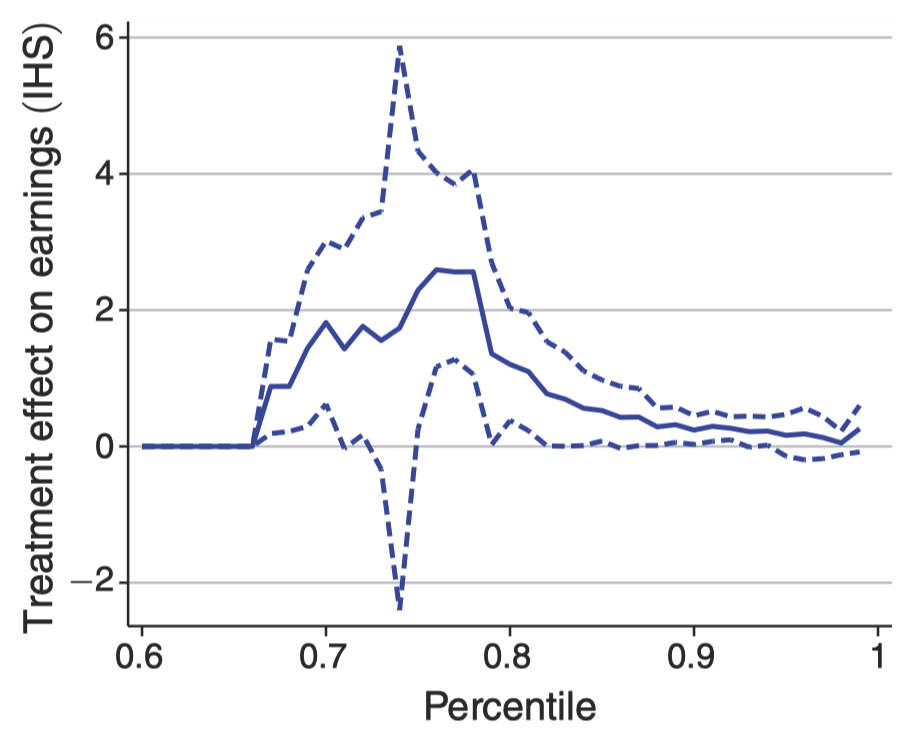
\includegraphics[width = 0.8 \textwidth]{images/quantile_reg.png}
            \end{figure}}
            
            
        \end{column}
    \end{columns}
    
\end{frame}

\begin{frame}{Intervention 1: Treatment Effect Decomposition}
    Does $V_{i,i}$ really increase? Another piece of evidence:
    \vspace*{-10pt}
    \begin{columns}[T]
        \begin{column}{0.45\textwidth}
            \begin{figure}
                \centering
                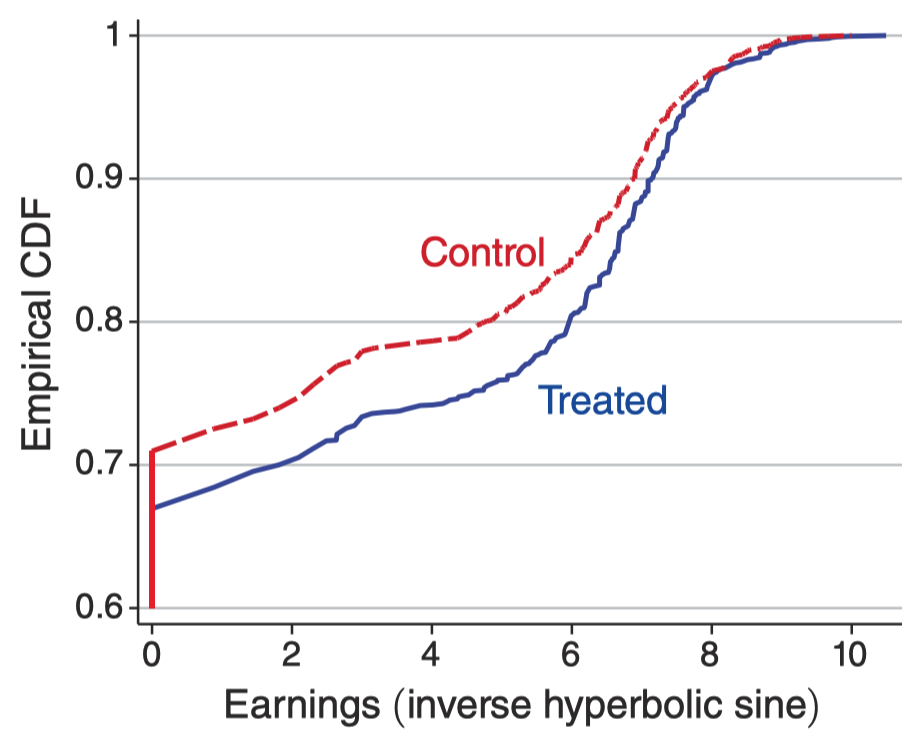
\includegraphics[height = 0.6 \textheight]{images/dist_earnings.png}
            \end{figure}
        \end{column}

        \begin{column}{0.45\textwidth}
            \begin{figure}
                \centering
                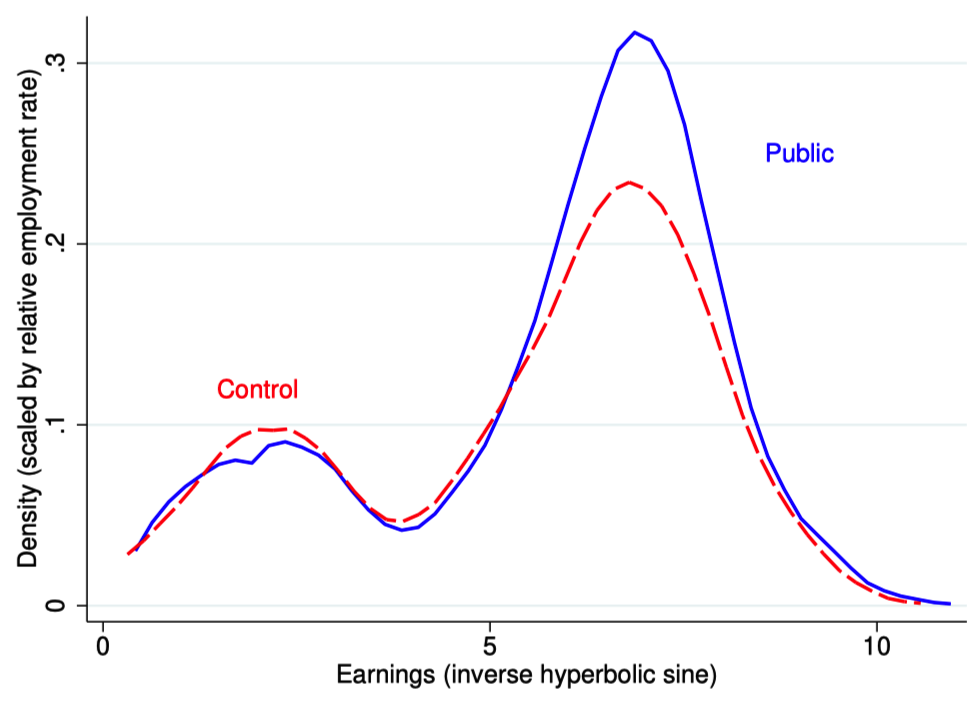
\includegraphics[height = 0.6 \textheight]{images/dist_earnings_empadj.png}
            \end{figure}
        \end{column}
    \end{columns}
\end{frame}

\begin{frame}{Intervention 1: Behavioral and Belief Changes of Workseekers}
    \begin{table}[h!]
        \scriptsize
        \begin{center}
            \begin{tabular}{lcccccccc}
            & {accurate} & {$>$ median} & targeted & used & applications & interviews & offers & expected \\
            & {belief} & {self-esteem} & search & report & w. report & w. report & w. report & offers \\
            \hline
            &\\
            public & \textcolor<1>{fuzzywuzzy!65!white}{$0.158^{***}$} & \textcolor<1>{fuzzywuzzy!65!white}{$0.002$} & \textcolor<2>{fuzzywuzzy!65!white}{$0.051^{***}$} & \textcolor<2>{fuzzywuzzy!65!white}{$0.699^{***}$} & \textcolor<2>{fuzzywuzzy!65!white}{$1.682^{***}$} & \textcolor<3>{fuzzywuzzy!65!white}{$0.432^{***}$} & \textcolor<3>{fuzzywuzzy!65!white}{$0.112^{***}$} & \textcolor<3>{fuzzywuzzy!65!white}{$0.106^{***}$} \\
            & {(0.008)} & {(0.013)} &(0.010) & (0.013) & (0.040) & (0.023) & (0.011) & (0.019)\\
             &\\
            mean (C) & {0.389} & 0.553 & 0.155 & 0.000 & 0.000 & 0.000 & 0.000 & 4.198
            \end{tabular}
        \end{center}
    \end{table}

    \begin{itemize}
        \item<1-> assessments \textit{correct} beliefs
        \item<2-> assessments are used for job searching
        \item<3-> assessments improve employment 
    \end{itemize}
\end{frame}

\begin{frame}{Intervention 1: Some Subtle Changes Are Happening}
    \begin{table}[h!]
        \footnotesize
        \begin{center}
            \begin{tabular}{lcccc}
            & {any} & {search} & search & No.  \\
            & {search} & {hours} & cost & applications  \\
            \hline
            &\\
            public & $\textcolor<2>{fuzzywuzzy!65!white}{-}0.020$ & {$\textcolor<2>{fuzzywuzzy!65!white}{-}0.036$} & {$\textcolor<2>{fuzzywuzzy!65!white}{-}0.094$} & {$0.019$}\\
            & {(0.014)} & {(0.048)} &(0.080) & (0.042) \\
             &\\
            mean (C) & {0.389} & 0.553 & 0.155 & 0.000 
            \end{tabular}
        \end{center}
    \end{table}
    Potentially,
    \begin{itemize}
        \small
        \item certification changes \underline{\textit{how}} workseekers search
        \item certification-induced changes may be \textit{\underline{temporary}}, hence not captured by the baseline survey
    \end{itemize}
\end{frame}

%\textcolor<1>{fuzzywuzzy!65!white}

\subsection*{Experiment II}
\begin{frame}{Intervention 2: \textit{Private} Certification}
    \begin{table}[h!]
        \scriptsize
        \begin{center}
            \begin{tabular}{lccc}
            
            & \multicolumn{2}{c}{{\textbf{report}}} & \multirow{2}{*}{{\textbf{no report}}} \\
            & {{\textit{shareable}}} & {\textit{non-shareable}} & \\
            \hline
            \multirow{2}{*}{\transparent{0.2}{\color{fuzzywuzzy!65!white} \underline{No. certified applicants}}} & \multicolumn{2}{c}{\transparent{0.2}?} & {0} \\
             & {{?}} & {?} & 
            \end{tabular}
        \end{center}
    \end{table}
    \vspace*{-5pt}
    \uncover{\only<1>{\begin{itemize}
        \small
        \item[\texthlit{T1}] email version, and 20+ colorered high-quality paper copies \texthlbf{with credibility}
    \end{itemize}}
    \only<2>{\begin{itemize}
        \small
        \item[\texthlit{T2}] {\underline{NO}} email version, and 1 \underline{black-and-white low-quality} paper copies \texthlbf{without credibility}
    \end{itemize}}

    \vspace*{-18pt}
    \begin{columns}[T]
        \begin{column}{0.4\textwidth}
            \only<1>{\begin{figure}
                \centering
                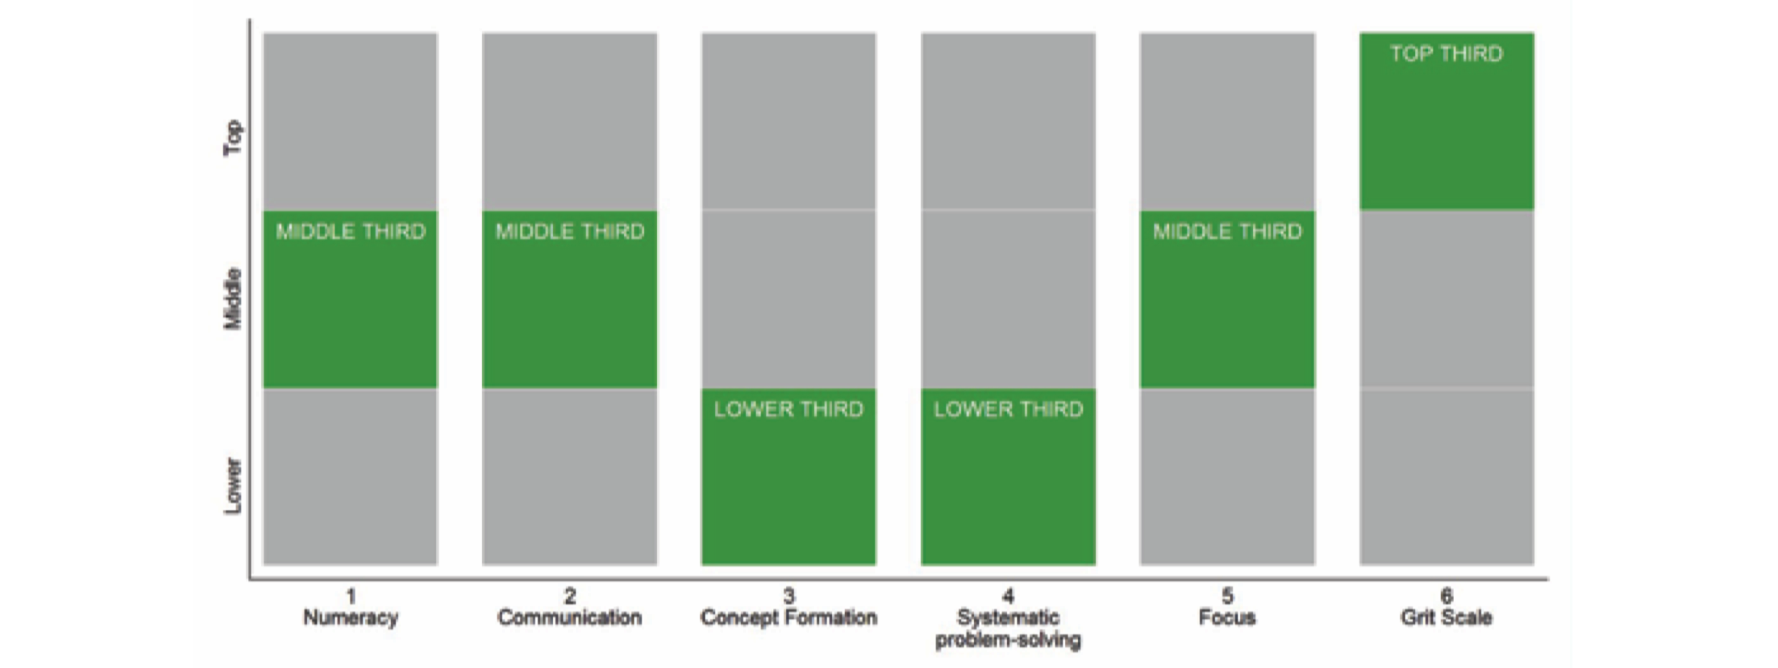
\includegraphics[width = 0.95 \textwidth]{images/T1_assess.png}
            \end{figure}}
            \only<2>{\begin{figure}
                \centering
                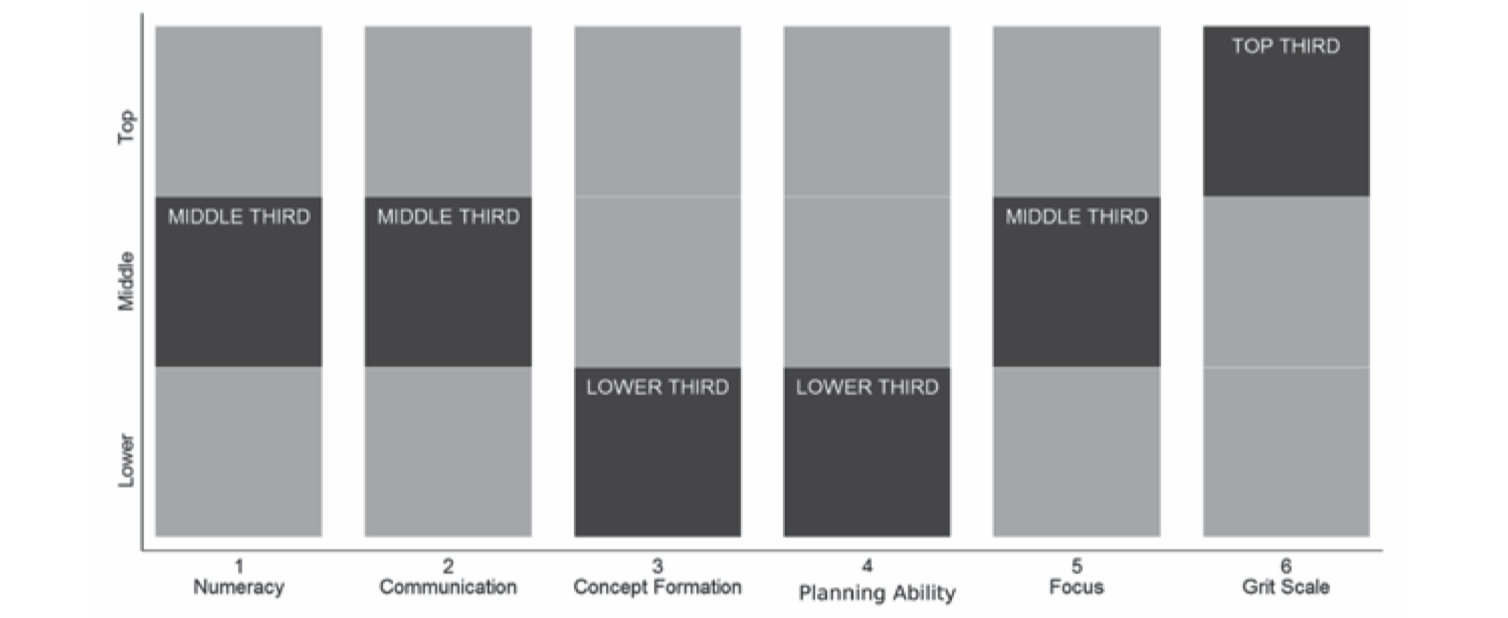
\includegraphics[width = 0.95 \textwidth]{images/T2_assess.png}
            \end{figure}}
        \end{column}

        \begin{column}{0.55\textwidth}
            \only<1>{\begin{figure}
                \centering
                
\includegraphics[width = 0.95 \textwidth]{images/T1_cert.png}
            \end{figure}}
            \only<2>{\begin{figure}
                \centering
                
\includegraphics[width = 0.95 \textwidth]{images/T2_cert.png}
            \end{figure}}

            \only<1>{
            \vspace*{-15pt}
            \begin{itemize}
                \footnotesize
                \item[-] assessments are carefully explained
                \item[-] encouraged to be used for job application
            \end{itemize}
            }
            \only<2>{
            \vspace*{-15pt}
            \begin{itemize}
                \footnotesize
                \item[-] assessments are \underline{still} carefully explained
                \item[-] \underline{NOT} encouraged to be used for job application
            \end{itemize}
            }
        \end{column}
    \end{columns}}
\end{frame}

\begin{frame}{Intervention 2: \textit{Private} Certification}
    \vspace*{-5pt}
    \begin{itemize}
        \small
        \item[\texthlit{T1}] {\underline{NO}} email version, and 1 \underline{black-and-white low-quality} paper copies \texthlbf{without credibility}
    \end{itemize}
    \begin{table}[h!]
        \small
        \begin{center}
            \begin{tabular}{lccc}
            
            & \multicolumn{2}{c}{{\textbf{report}}} & \multirow{2}{*}{{\textbf{no report}}} \\
            & {{\textit{shareable}}} & {\textit{non-shareable}} & \\
            \hline
            \multirow{2}{*}{\transparent{0.2}{\color{fuzzywuzzy!65!white} \underline{No. certified applicants}}} & \multicolumn{2}{c}{\transparent{0.2}?} & {0} \\
             & {{?}} & {?} & \\ \hline \hline
            N & \multicolumn{2}{c}{\transparent{0.2}\textbf{2247}} & {\textbf{2274}}\\
            & \textit{2247} & \textit{2114} & 
            \end{tabular}
        \end{center}
    \end{table}
    
\end{frame}

\begin{frame}{Intervention 2: Behavioral and Belief Changes of Workseekers}
    \begin{table}[h!]
        \scriptsize
        \begin{center}
            \begin{tabular}{lcccccccc}
            & {accurate} & {$>$ median} & targeted & used & applications & interviews & offers & expected \\
            & {belief} & {self-esteem} & search & report & w. report & w. report & w. report & offers \\
            \hline
            &\\
            public & \textcolor<1>{fuzzywuzzy!65!white}{$0.158^{***}$} & \textcolor<1>{fuzzywuzzy!65!white}{$0.002$} & \textcolor<2>{fuzzywuzzy!65!white}{$0.051^{***}$} & \textcolor<2>{fuzzywuzzy!65!white}{$0.699^{***}$} & \textcolor<2>{fuzzywuzzy!65!white}{$1.682^{***}$} & \textcolor<3>{fuzzywuzzy!65!white}{$0.432^{***}$} & \textcolor<3>{fuzzywuzzy!65!white}{$0.112^{***}$} & \textcolor<3>{fuzzywuzzy!65!white}{$0.106^{***}$} \\
            & {(0.008)} & {(0.013)} &(0.010) & (0.013) & (0.040) & (0.023) & (0.011) & (0.019)\\
            private & \textcolor<1>{fuzzywuzzy!65!white}{$0.123^{***}$} & \textcolor<1>{fuzzywuzzy!65!white}{$-0.002$} & \textcolor<2>{fuzzywuzzy!65!white}{$0.047^{***}$} & \textcolor<2>{fuzzywuzzy!65!white}{$0.290^{***}$} & \textcolor<2>{fuzzywuzzy!65!white}{$0.572^{***}$} & \textcolor<3>{fuzzywuzzy!65!white}{$0.144^{***}$} & \textcolor<3>{fuzzywuzzy!65!white}{$0.036^{***}$} & \textcolor<3>{fuzzywuzzy!65!white}{$0.054^{***}$} \\
            & {(0.008)} & {(0.015)} &(0.010) & (0.012) & (0.033) & (0.017) & (0.008) & (0.023)\\
             &\\
            $p_{\text{public=private}}$ & \textcolor<1>{fuzzywuzzy!65!white}{$0.000^{***}$} & \textcolor<1>{fuzzywuzzy!65!white}{$\boxed{0.812}$} & \textcolor<2>{fuzzywuzzy!65!white}{$\boxed{0.701}$} & \textcolor<2>{fuzzywuzzy!65!white}{$0.000^{***}$} & \textcolor<2>{fuzzywuzzy!65!white}{$0.000^{***}$} & \textcolor<3>{fuzzywuzzy!65!white}{$0.000^{***}$} & \textcolor<3>{fuzzywuzzy!65!white}{$0.000^{***}$} & \textcolor<3>{fuzzywuzzy!65!white}{$0.025^{**}$} \\ 
            &\\
            mean (C) & {0.389} & 0.553 & 0.155 & 0.000 & 0.000 & 0.000 & 0.000 & 4.198
            \end{tabular}
        \end{center}
    \end{table}
\end{frame}

\begin{frame}{Intervention 2: What About The Subtle Changes?}
    \begin{table}[h!]
        \footnotesize
        \begin{center}
            \begin{tabular}{lcccc}
            & {any} & {search} & search & No.  \\
            & {search} & {hours} & cost & applications  \\
            \hline
            &\\ %\textcolor<2->{fuzzywuzzy!65!white}
            public & $\textcolor<1>{fuzzywuzzy!65!white}{-0.020}$ & {${-0.036}$} & {$\textcolor<1>{fuzzywuzzy!65!white}{-0.094}$} & {$0.019$}\\
            & {(0.014)} & {(0.048)} &(0.080) & (0.042) \\
            private & $\textcolor{fuzzywuzzy!65!white}{-0.006}$ & {$-0.036$} & {$\textcolor<1>{fuzzywuzzy!65!white}{-0.033}$} & {$0.037$}\\
            & {(0.014)} & {(0.049)} &(0.088) & (0.038) \\
             &\\
             $p_{\text{public=private}}$ & 1.000 & 1.000 & 1.000 & 1.000 \\
             &\\
            mean (C) & {0.389} & 0.553 & 0.155 & 0.000 
            \end{tabular}
        \end{center}
    \end{table}
\end{frame}

\begin{frame}{Intervention 2: Treatment Effects}
    \begin{table}[h!]
        \scriptsize
        \begin{center}
            \begin{tabular}{lccccc}
            & Employed & Hours & Earnings & Hourly wage & Written contract \\
            \hline
            \multicolumn{3}{l}{\texthlit{Total effect}} \\
            public & ${0.052^{***}}$ & {$0.201^{***}$} & {$0.337^{***}$} & {$0.197^{***}$} & {$0.020^{**}$}\\
            \uncover<2->{private & {$0.011$} & $0.066$ & $0.162^{**}$ & $0.094^{**}$ & $0.017^*$} \\
            \only<2>{public $\neq$ private & $0.002^{***}$ & $0.011^{**}$ & $0.028^{**}$ & $0.030^{**}$ & 0.769 \\}
            & \\
            \multicolumn{3}{l}{\texthlit{Extensive margin}} \\
            \uncover<1->{public & & $0.188^{***}$ & $0.269^{***}$ & $0.141^{***}$ & $0.020^{***}$ }\\
            \uncover<3->{private & & $0.041$ & $0.058$ & $0.030$ & $0.004$ }\\
            \only<3>{public $\neq$ private & & $0.001^{***}$ & $0.001^{***}$ & $0.001^{***}$ & $0.001^{***}$ \\}
            & \\
            \multicolumn{3}{l}{\texthlit{Intensive margin}} \\
            \uncover<1->{public & & $0.013$ & $0.069^*$ & $0.056^{**}$ & $-0.000$}\\
            \uncover<4->{private & & $0.025$ & $0.103^{***}$ & $0.064^{***}$ & $0.013^*$}\\
            \only<4>{public $\neq$ private & & $0.529$ & $0.380$ & $0.791$ & $0.102$ \\}
            & \\
            \multicolumn{3}{l}{\texthlit{Treatment effect $\mid$ employed}} \\
            \uncover<1->{public &  & $0.037$ & $0.194^{*}$ & $0.158^{**}$ & $-0.001$ }\\
            \uncover<5->{private &  & $0.083$ & $0.339^{***}$ & $0.209^{**}$ & $0.041^*$}\\
            \only<5>{public $\neq$ private & & $0.440$ & $0.234$ & $0.585$ & $0.078^*$}
            \end{tabular}
        \end{center}
    \end{table}
\end{frame}

\begin{frame}{Intervention 2: Treatment Effect Decomposition}
    \begin{columns}[T]
        \begin{column}{0.45\textwidth}
            \begin{figure}
                \centering
                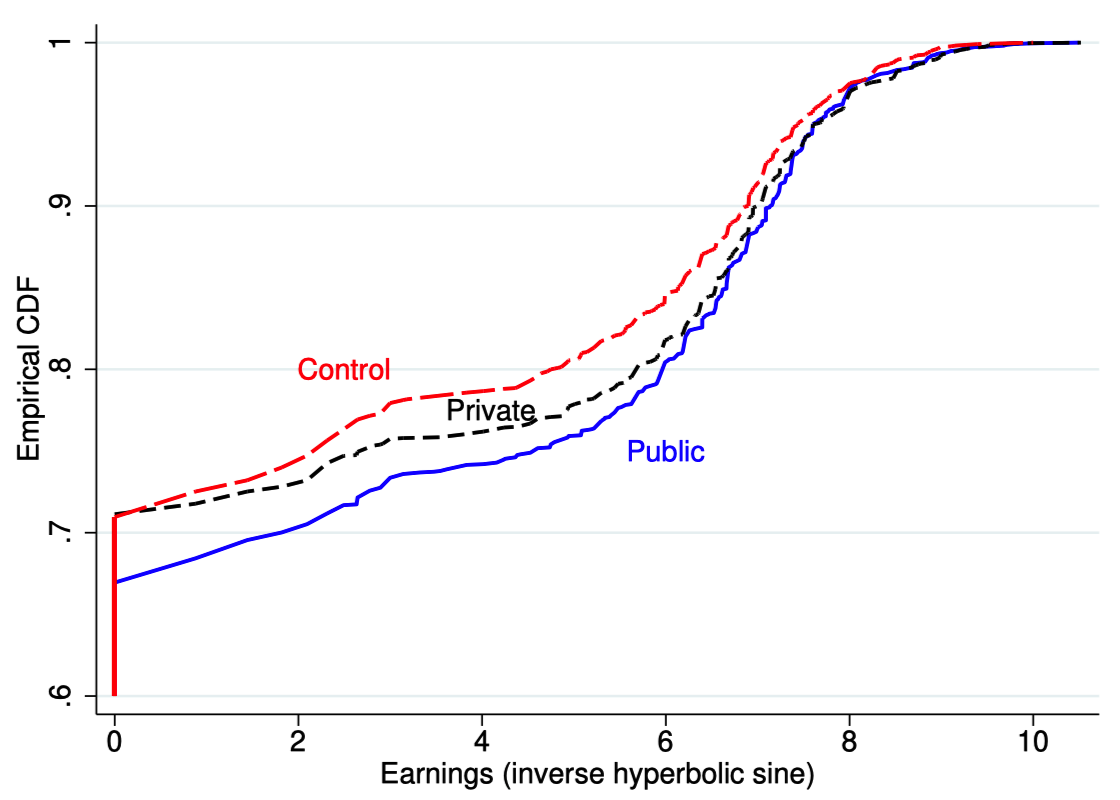
\includegraphics[width = 0.95 \textwidth]{images/T2_dist.png}
            \end{figure}
        \end{column}

        \begin{column}{0.45\textwidth}
            \begin{figure}
                \centering
                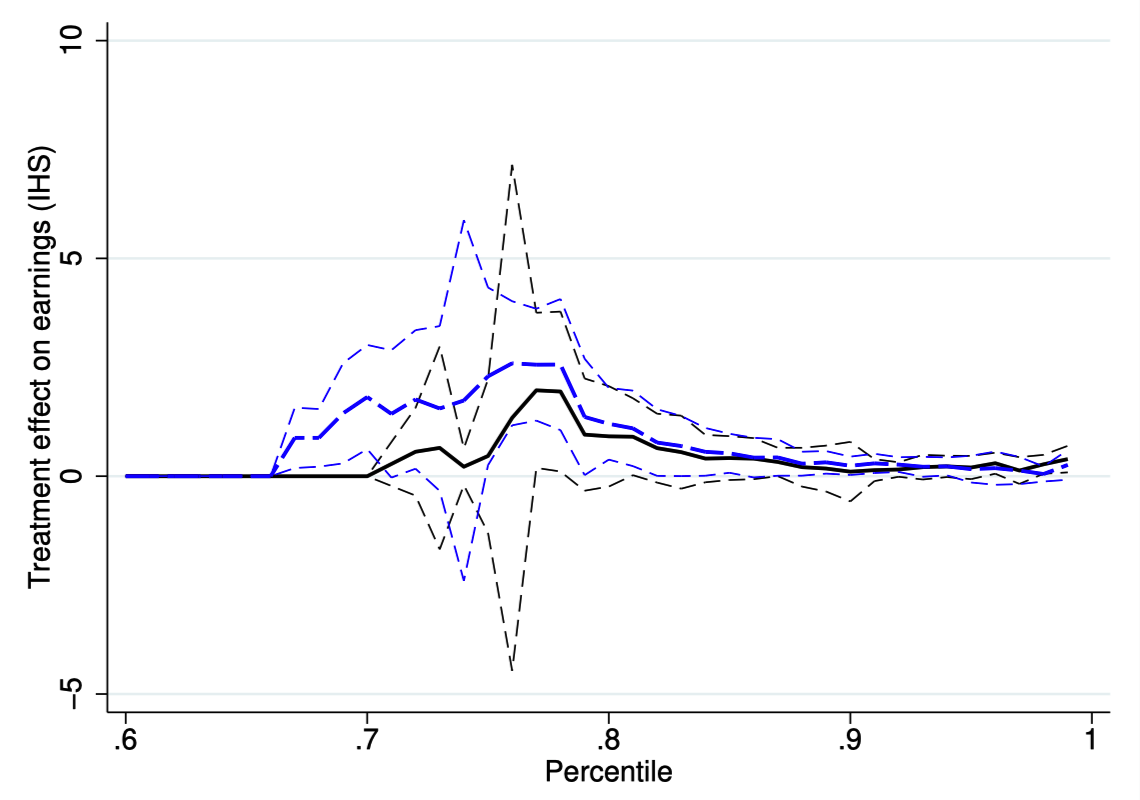
\includegraphics[width = 0.95 \textwidth]{images/T2_quanttreat.png}
            \end{figure}
        \end{column}
    \end{columns}

    \vspace*{10pt}
    \texthlit{Intensive margins} matter \textit{more} for the private treatment.
    \vspace*{10pt}
\end{frame}
